A Point-Of-Presence (POP) is an artificial demarcation point or interface point between communicating entities.
In our case we are referring to optical fiber interconnection points.
From 2010 until now the guifi.net community has raised six points of presence over the Catalan territory.
This POPs are following the network model of freedom and neutrality specified in the community network license\footnote{This is the agreement all users must accept to join the network. It's mission is to keep the network free, open and neutral. The Catalan version can be found at \url{http://guifi.net/ca/CXOLN}. It has not yet been translated into English}.
Thus anyone is able to connect to them but always respecting the same conditions.

From a general perspective guifi.net community is building a set of neutral exchange points, leaving the
infrastructure available to the individuals, associations or either companies. These kind of POPs are named POP-IX making
reference to the internet exchange points (IX).

Figure \ref{fig:fibre_map} shows the fiber network map of guifi.net POPs (not all of them).

The current guifi.net POPs are managed, maintained and also economically sustained for the community. 
To interconnect all of them it is need to use third party infrastructure. The FFTH projects are able to deploy some kilometres
of optical fiber but not hundreds or even thousands.

In Catalonia there exist a set of deployed fibers which are owned by the Catalan government, available to any entity and 
rented for a regularized price. Most of the guifi.net POPs are connected to such network to interchange data
between them. Figure \ref{fig:xoc_map} shows a slice of the network fiber map provided by the government. 

\begin{figure}[htbp]
  \centering
  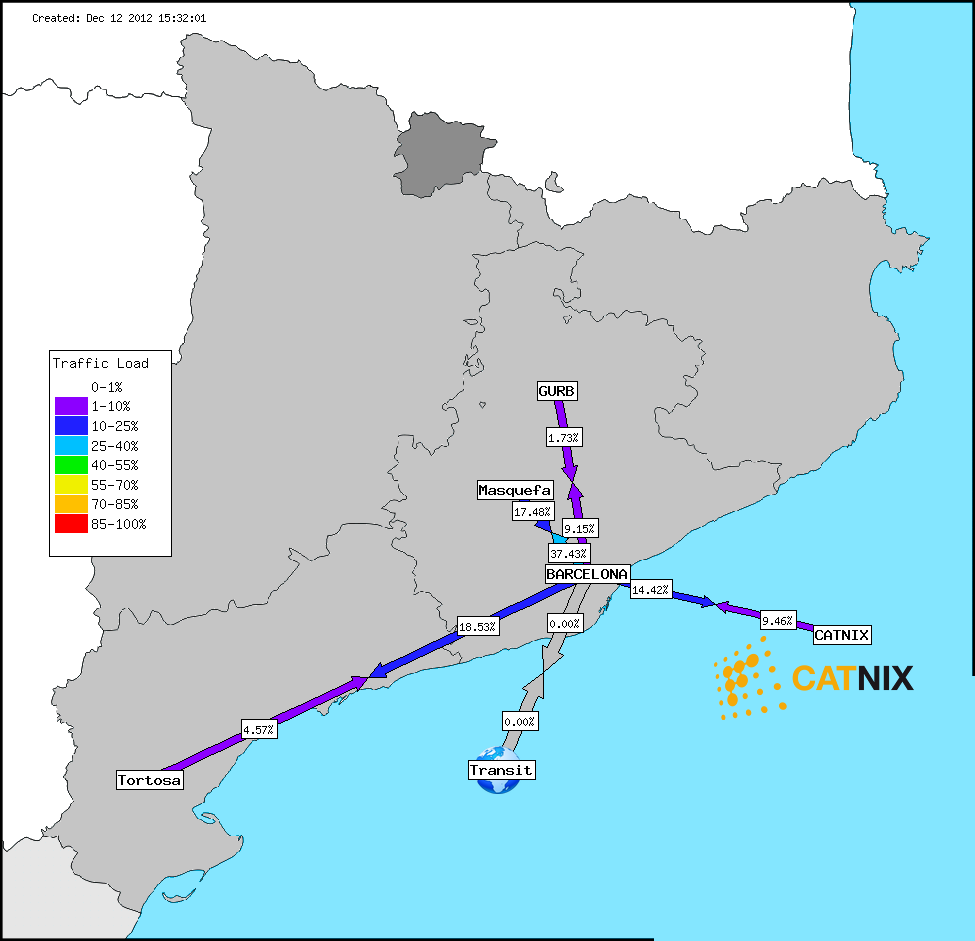
\includegraphics[scale=.35]{sect3/figures/pops_network_map.eps} 
  \caption{Guifi.net fiber POPs network map}
  \label{fig:fibre_map}
\end{figure}

\begin{figure}[htbp]
  \centering
  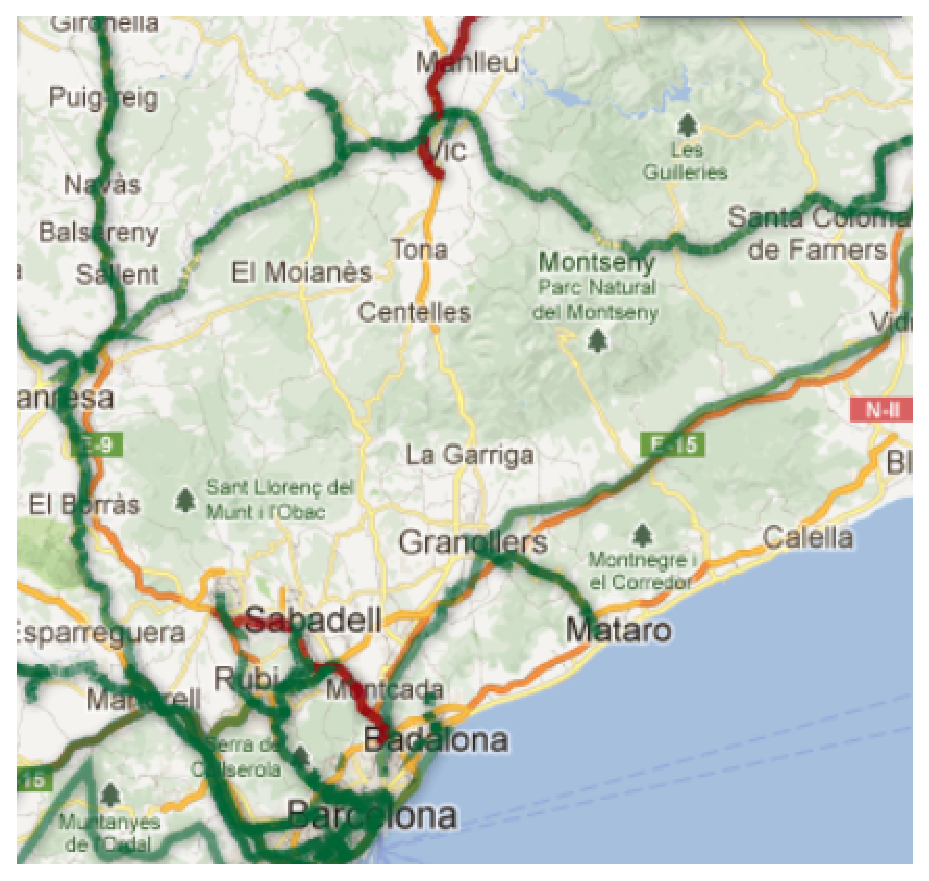
\includegraphics[scale=.5]{sect3/figures/xoc_map.eps} 
  \caption{Available regularized fiber}
  \label{fig:xoc_map}
\end{figure}


\FloatBarrier
\subsection{Pilot's POPs}

\FloatBarrier
\subsubsection{Gurb}
Gurb is a small village in a rural area of the geographical center of Catalonia. Back in 2004 the first guifi.net community
was born here. Probably because of that Gurb is nowadays one of the places where the bottom-up broadband model has more
influence. As explained in Section~\ref{sec:deployments} the community users deployed some optical fiber kilometres to reach the government
infrastructure and connect with other POPs.


It is a very important point-of-presence because it allows a small data center provided and maintained by the community.
There are even ISP companies connected to such POP following and using the open-network model to provide Internet
connectivity to end users.


\begin{figure}[htbp]
  \centering
  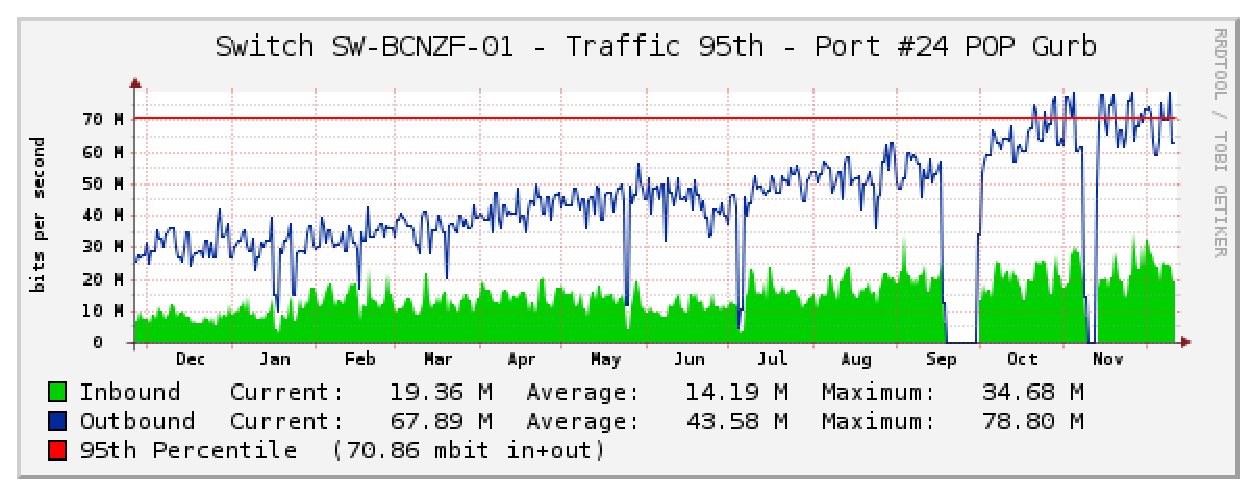
\includegraphics[scale=.65]{sect3/figures/gurb_network_load_year.eps} 
  \caption{Gurb's POP network load (year 2012).}
  \label{fig:gurb_net_load}
\end{figure}



\FloatBarrier
\subsubsection{Vic}



\begin{figure}[htbp]
  \centering
  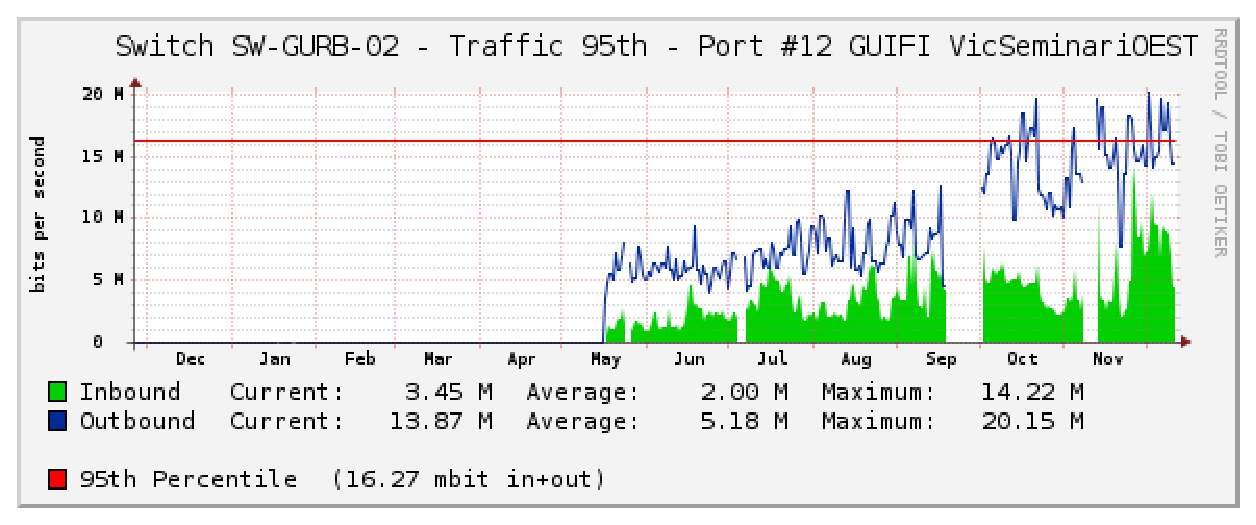
\includegraphics[scale=.65]{sect3/figures/vic_network_load_year.eps} 
  \caption{Vic's POP network load (year 2012).}
  \label{fig:vic_net_load}
\end{figure}



\FloatBarrier
\subsection{Other POPs}

Other points-of-present not directly related with this project are:

\begin{itemize}
	\item Masquefa: blablabla IGLU?

	\item Tortosa: It is a city placed on the sud of Catalonia. The guifi.net users started a goverment's funded project named 
		OpenFPnet\footnote{\url{http://openfpnet.guifi.net}} which tries to create an open and neutral fiber backbone 
		around the zone and the surrounding villages. Starting from that point they opened a POP to connect with the 
		rest of guifi.net infrastructure. Currently this point-of-presence is economically maintained by some community 
		users grouped in associations and some company with interests of use such fiber.

	\item Barcelona: The Catalonia's capital POP is the one placed in the Internet exchange point CATNIX.
\end{itemize}

\FloatBarrier
\subsubsection{Telvent-Barcelona}

Telvent-Barcelona is a commercial data center of Telvent\footnote{\url{http://www.telvent.es/en/}} placed in an industrial park of Barcelona. It hosts CATNIX\footnote{\url{http://www.catnix.net}}, the Internet exchange point (IX) of Catalonia, a physical infrastructure provided by the Catalan government. IXs are critical for the Internet since they are meant to let the network operators exchange their information and connect their networks (autonomous systems). 

On the one hand, as be shown in Figure \ref{fig:fibre_map}, all guifi.net POPs are linked to TELVENT-Barcelona. On the other hand, guifi.net connects to the Internet through this POP.

guifi.net Foundation operates it's own backbone infrastructure using the ASN 49835 (Autonomous System Number). 
An open peering policy is followed to establish peering sessions with all potential partners. Figure~\ref{fig:catnix_net_load} shows the total peering traffic. Additionally guifi.net Foundation has an Internet Gigabit uplink contracted with Cogent\footnote{\url{http://www.cogentco.com/en/}}. Figure~\ref{fig:cogent_load} . All guifi.net Foundation routers and servers are allocated in a 22U rack in Telvent-Barcelona, shown in Figure~\ref{fig:telvent_rack}. 


Figure \ref{fig:telvent_scheme} shows a connection scheme (layer 2) of the hardware used for the CATNIX POP. 
The first port of the switch SW-03 is the optical fiber which brings the data from the other POPs. As can be seen each
of them use a separate VLAN. The seventh port of the second switch is the connection with the carrier to reach the Internet.
And the eight is connected to the CATNIX infrastructure where the exchange of data with other ISPs and networks is possible. 


The Telvent-Barcelona Foundation resources are shared with other partners, such as puntCat\footnote{\url{http://www.domini.cat/}}, the Catalan Top-Level Domain (TDL), which is currently using half of the space available.

\begin{figure}[htbp]
  \centering
  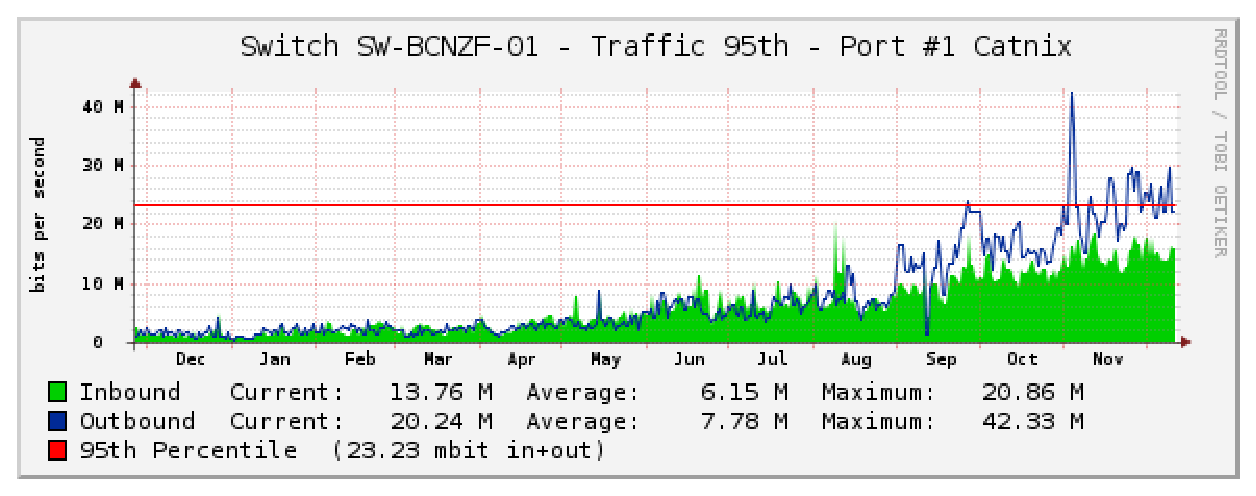
\includegraphics[scale=.65]{sect3/figures/catnix_network_load_year.eps} 
  \caption{Telvent-Barcelona's POP network load (year 2012).}
  \label{fig:catnix_net_load}
\end{figure}


\begin{figure}[htbp]
  \centering
  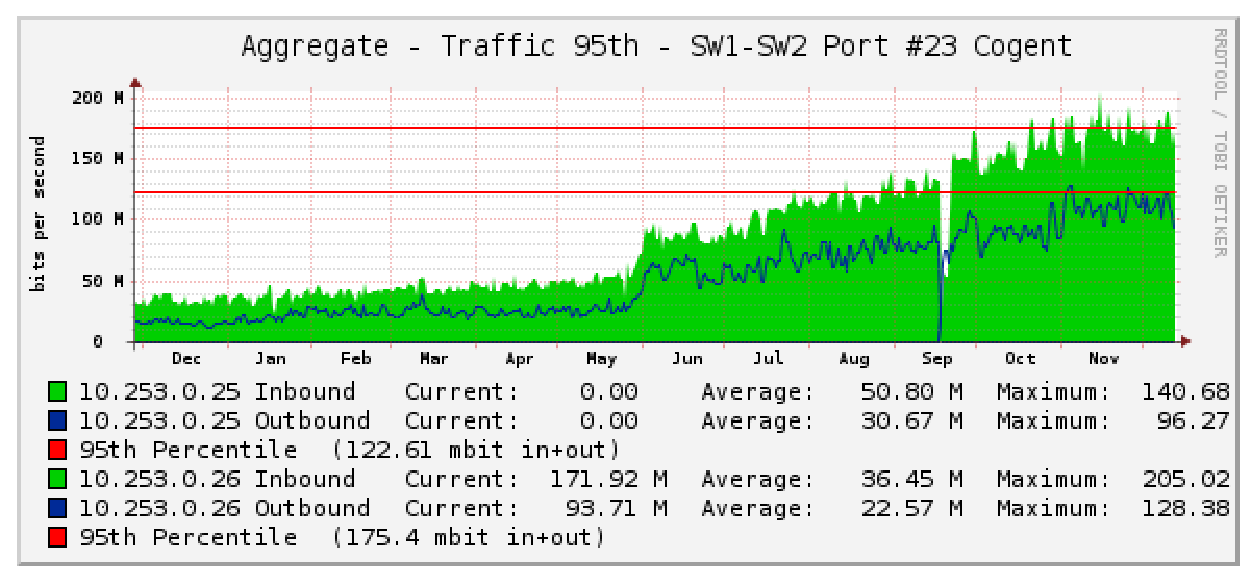
\includegraphics[scale=.65]{sect3/figures/cogent_network_load2.eps} 
  \caption{Internet uplink load (year 2012).}
  \label{fig:cogent_load}
\end{figure}


\begin{figure}[htbp]
  \centering
  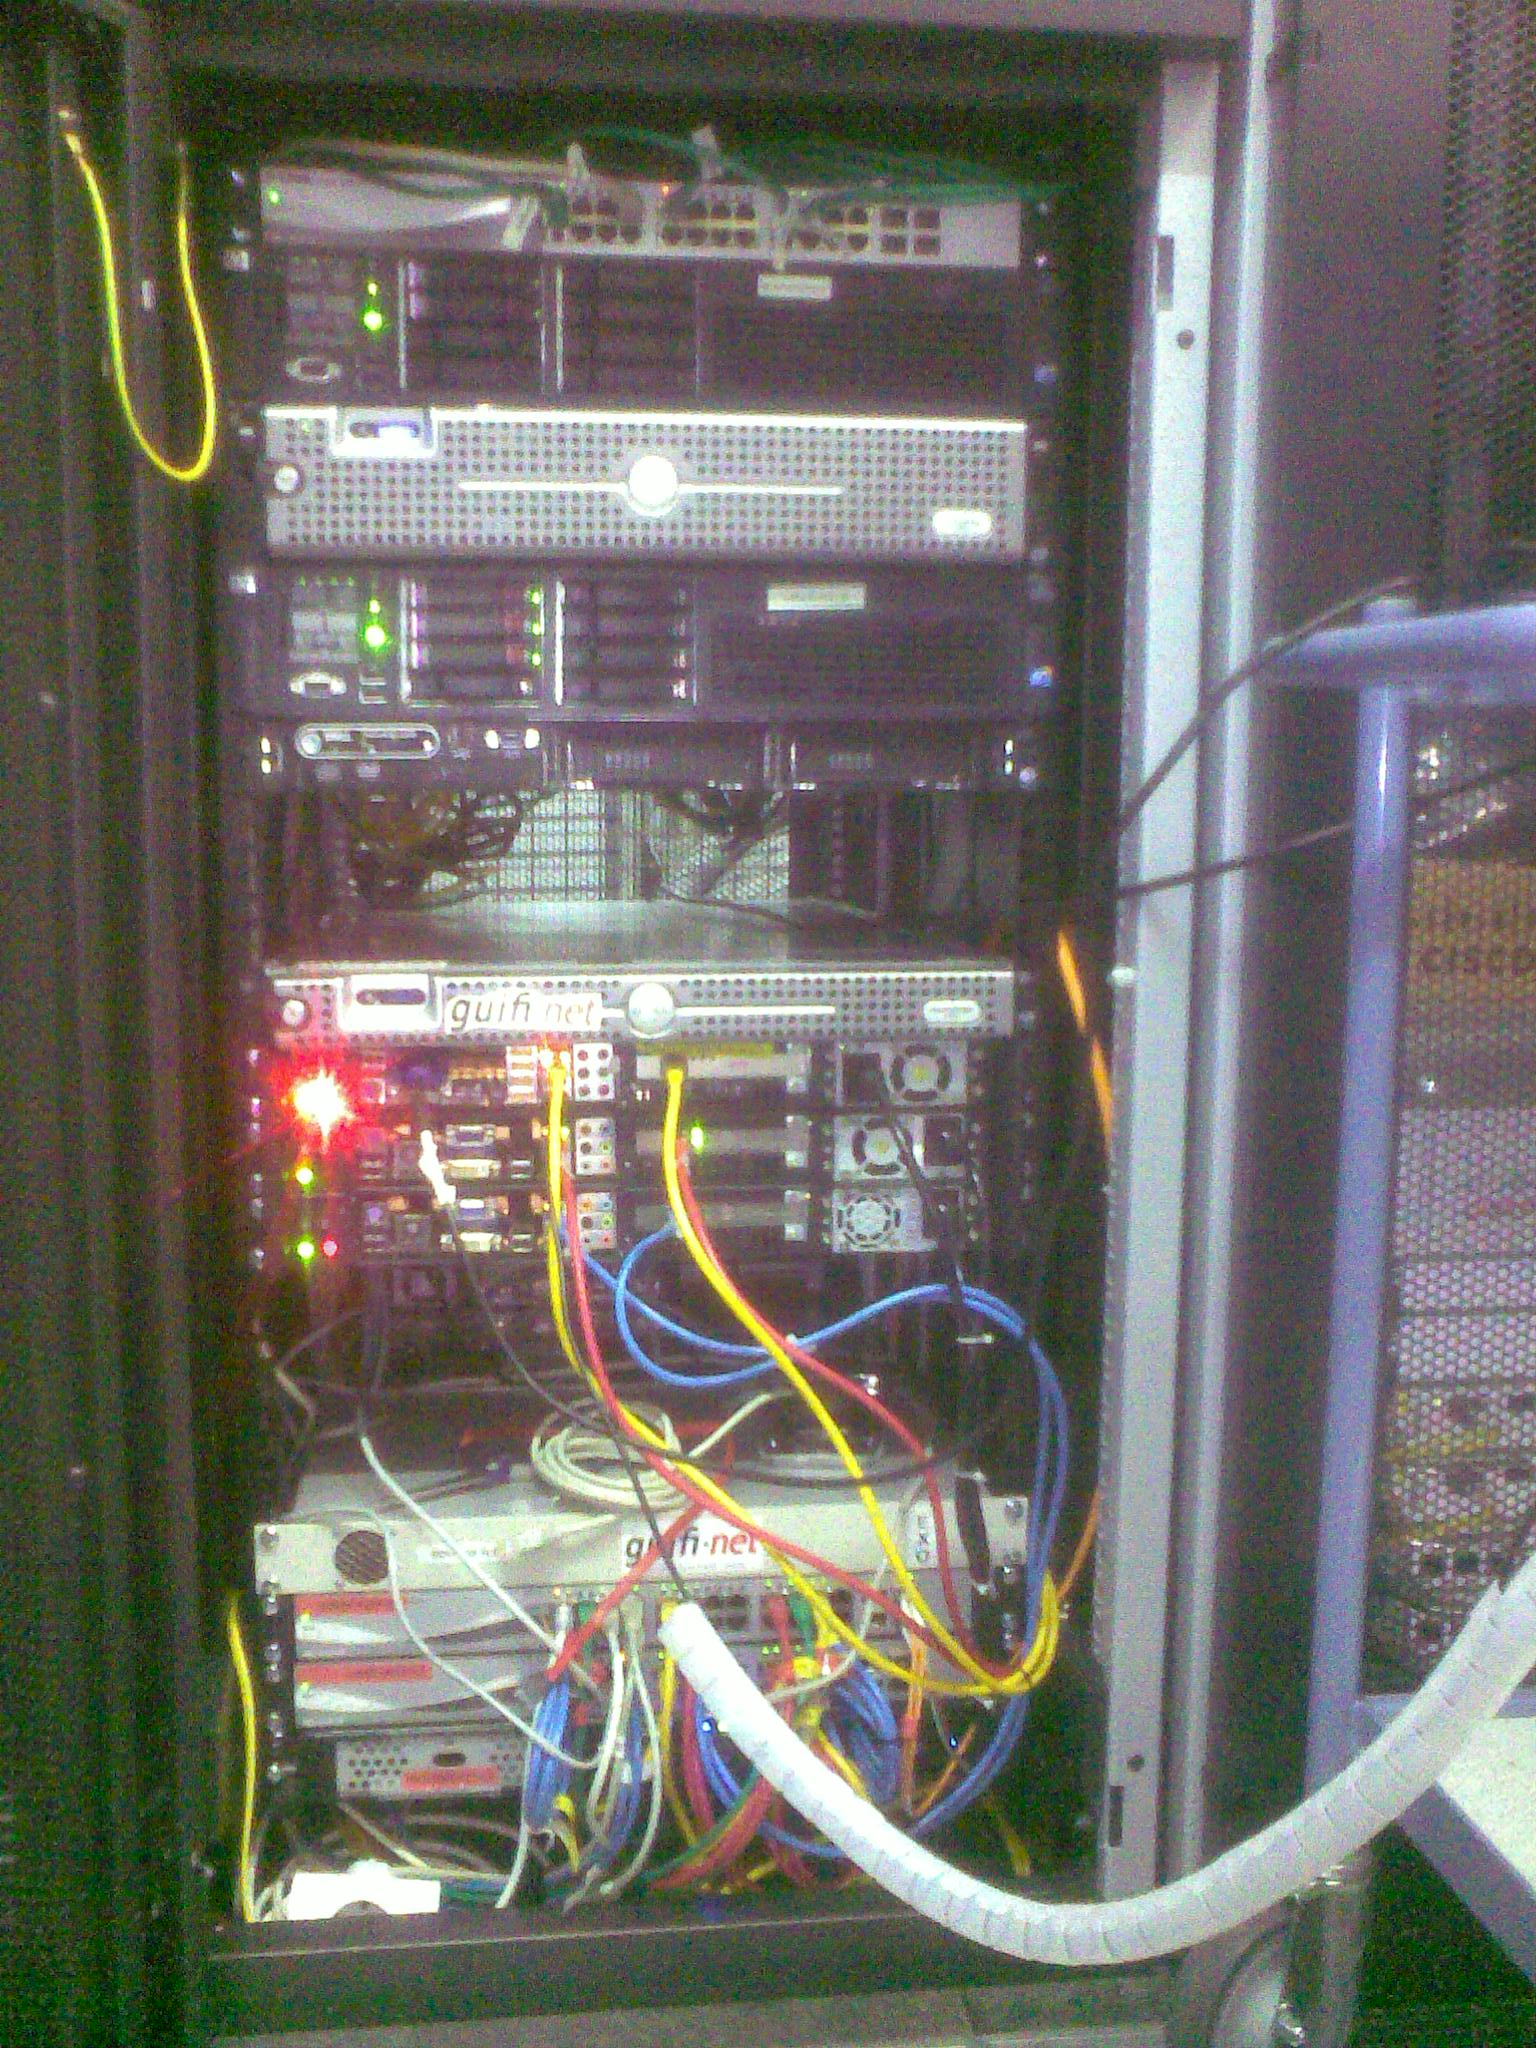
\includegraphics[scale=.65]{sect3/figures/telvent_rack_front_view.eps} 
  \caption{guifi.net Foundation rack in TELVENT-Barcelona.}
  \label{fig:telvent_rack}
\end{figure}


\begin{figure}[htbp]
  \centering
  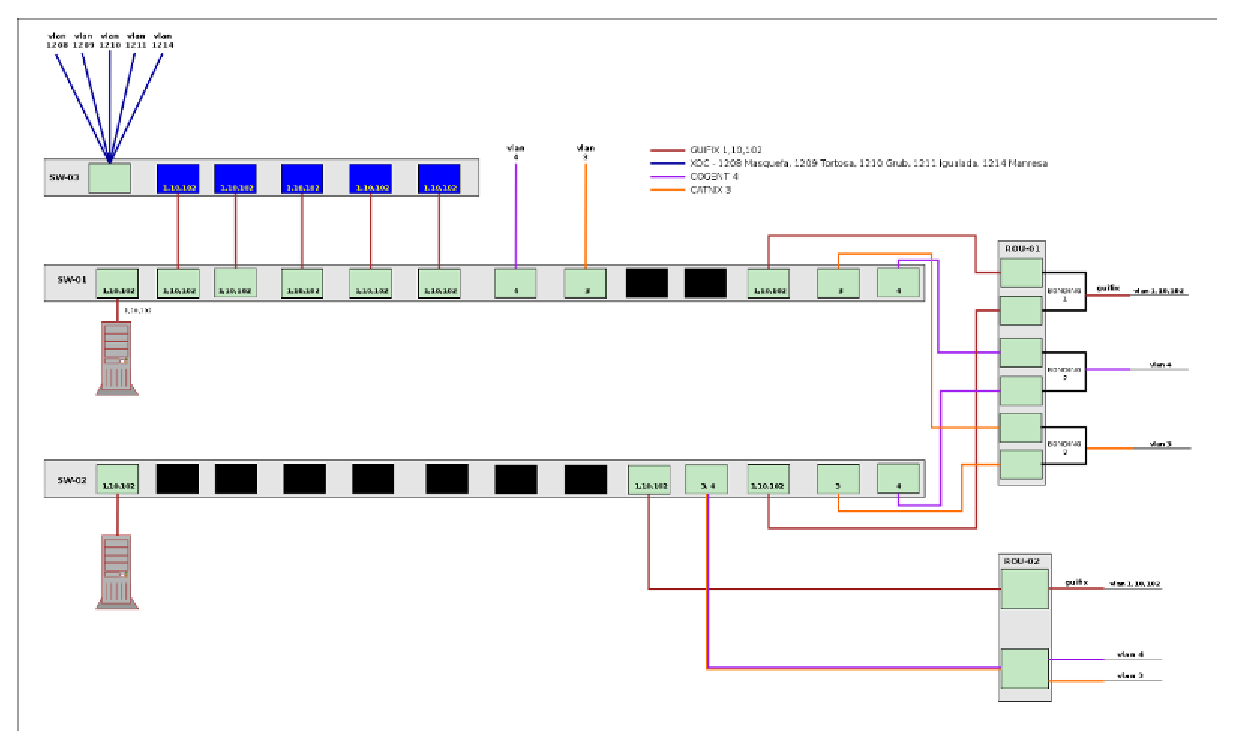
\includegraphics[scale=.75]{sect3/figures/telvent_scheme.eps} 
  \caption{CATNIX connections scheme}
  \label{fig:telvent_scheme}
\end{figure}



\FloatBarrier
\subsubsection{Tortosa}
Tortosa is a city placed on the south of Catalonia. The guifi.net users started a project named 
OpenFPnet\footnote{\url{http://openfpnet.guifi.net}} with the objective of create an open and neutral fiber backbone 
around the surrounding villages. This project was initially partially-funded by the government. 
\newline
Starting from that point they opened a POP to connect with the rest of guifi.net infrastructure. 
Currently it is economically sustained by community users grouped in associations and some company with interests in use
this open and neutral point.


\FloatBarrier
\subsubsection{Masquefa}

